\chapter{Marco Teórico}\label{cap3:Marco-Teorico}

\section{Función logística}

La regresión logística es uno de los primeros algoritmos utilizados para resolver 
problemas de clasificación. Aunque su nombre pueda llevar a confusión al incluir la 
palabra ''Regresión'', este algoritmo no se emplea para problemas de regresión, sino 
para clasificación. Se aplica comúnmente en problemas de clasificación binaria 
\cite{Brownlee} Pág. 57. \medskip

La regresión logística es una técnica adecuada para clasificar si un cliente 
será un buen pagador debido a varias razones:

\begin{itemize}
    \item Es ideal para predecir dos posibles resultados, como ''buen pagador o mal pagador'' , ''confiable o no confiable''.
    \item Permite entender cómo diferentes características afectan la probabilidad de que un cliente sea "confiable o no confiable".
    \item No solo clasifica a los clientes, sino que también proporciona una probabilidad de que sean buenos pagadores, lo que facilita la toma de decisiones basadas en riesgo.
    \item Es un método rápido y eficiente para grandes volúmenes de datos.
\end{itemize}



La función logística \cite{Brownlee} Pág. 52, también conocida como la 
función sigmoide, es una función matemática comúnmente utilizada en
problemas de clasificación. Su forma característica es una curva en forma 
de ''S'' que transforma cualquier número real en un rango entre 0 y 1. \medskip


La función logística esta definida de la siguiente manera:

$$ \displaystyle y=logit(x)= \frac{1}{1+e^{-x}} $$


Y la grafica es: 

\begin{figure}[H]
    \centering
       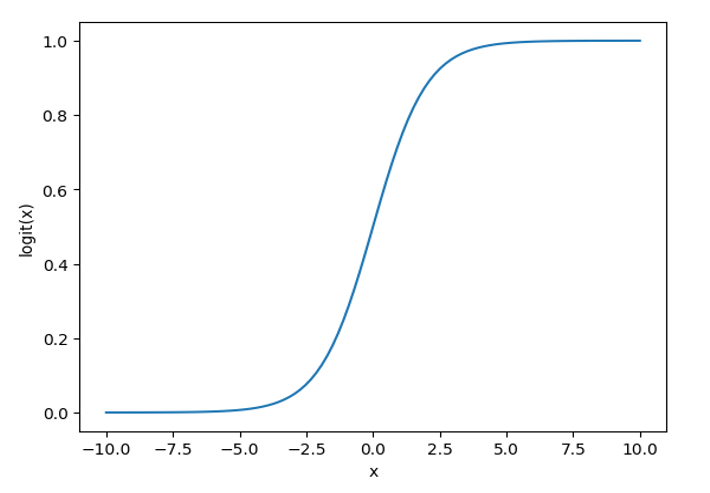
\includegraphics[width=12cm, height=7cm ]{Imagenes/Logit.PNG}
      \caption{Función logística , realizada en Scikit-Learn}
      \label{fig:logit}
  \end{figure} 

Esta claro que $ \displaystyle x \in ( \infty , {-}\infty ) \;  y \; logit(x) \in [0 , 1]$ \medskip
En general nuestra ecuación de trabajo será de la siguiente forma : \medskip

$$ \displaystyle y=B_0 + B_1X_1 + B_2X_2+ \dots + B_nX_n $$

 
Ahora tenemos muchos puntos de datos, por decir m puntos de datos en nuestro dataset. Para cada
punto de datos tendremos : \medskip

$$\displaystyle \sigma (y_i)= \frac{1}{1+e^{-y_i}} = \frac{1}{1+e^{-(B_0 + B_1X_{1i} + B_2X_{2i}+ \dots + B_nX_{ni})}} $$ \medskip

 Entonces,para cada punto, obtenemos un valor entre 0 y 1. Para hacer las preddicciones
 usamos el siguiente criterio: \medskip

\[
y = \left\{ \begin{array}{lcl}
1 & \mbox{ si } & \sigma (y) > 0.5 \\
& & \\
0 & \mbox{ si } & \sigma (y) \leq 0.5
\end{array}
\right.
\] \medskip

 Vamos a llamar $\sigma(y_i)$ como $p_i$ \\
 $$\displaystyle p_i =\widehat{y_i} = \sigma (y_i)= \frac{1}{1+e^{-y_i}} = \frac{1}{1+e^{-(B_0 + B_1X_{1i} + B_2X_{2i}+ \dots + B_nX_{ni})}} $$ \medskip
 
 \begin{itemize}
    \item $\displaystyle p_i = 1$ es la probabilidad de que la variable dependiente $\sigma (y_i)$ sea igual a 1 .
    \item $\displaystyle B_0 , B_1, B_2 , \dots,B_n$ son los parametros del modelo.
    \item $\displaystyle X_0 , X_{i1}, X_{i2} , \dots,X_{in}$ son las variables independientes del modelo.    
\end{itemize}

\section{Estimador de máxima verosimilitud}

Si tenemos n observaciones y para cada observación tenemos \medskip

$$ P(y_i =1 ) = \widehat{y_{i}}= \frac{1}{1+e^{-y_i}} = \frac{1}{1+e^{-(B_0 + B_1X_{1i} + B_2X_{2i}+ \dots + B_nX_{ni})}} $$  \medskip

Y la probabilidad de que $ y_i = 0 $ es:\medskip

$$ P(y_i =1 ) = \widehat{y_{i}}= \frac{1}{1+e^{-y_i}} = \frac{e^{(B_0 + B_1X_{1i} + B_2X_{2i}+ \dots + B_nX_{ni})}}{1+e^{(B_0 + B_1X_{1i} + B_2X_{2i}+ \dots + B_nX_{ni})}} $$  \medskip

La función de verosimilitud conjunta para todas las observaciones es: \medskip

$$ L(B_0 , B_1, B_2 , \dots,B_n) = \prod_{{i=1}}^{n} {\widehat{y_i}^{y_i}(1- \widehat{y_i})^{1- y_i}} $$ \medskip

Para simplificar la maximización, trabajamos con la log-verosimilitud , que es mas facil de manejar, Entonces \medskip

$$  \ell = ln(L(B_0 , B_1, B_2 , \dots,B_n)) =  ln(\prod_{i=1}^{n} \widehat{y_i}^{y_i}(1- \widehat{y_i})^{1- y_i}) = \sum_{i=1}^{n} (y_i ln(\widehat{y_i})+(1-y_i)ln(1- \widehat{y_i})) $$  \medskip

Para encontrar los estimadores de máxima verosimilitud, debemos maximizar la función 
log-verosimilitud con respecto a los parametros $(B_0 , B_1, B_2 , \dots,B_n)$ . Esto se logra calculando
las derivadas parciales de $ln$ con respecto a cada parámetro e igualando a cero:

$$ \frac{\delta \ell}{\delta B_j} =0 \, , \, para \, j\, =\, 0,1,\dots,n $$ \medskip

La derivada parcial con respecto a $B_0$ es \medskip

$$ \frac{\delta \ell}{\delta B_0} = \sum_{i=1}^{n} \displaystyle{\left(y_i - \frac{e^{(B_0 + B_1X_{1i} + B_2X_{2i}+ \dots + B_nX_{ni})}}{1+e^{(B_0 + B_1X_{1i} + B_2X_{2i}+ \dots + B_nX_{ni})}}\right)} $$ \medskip
Simplificando tenemos \\
$$ \frac{\delta \ell}{\delta B_0} = \sum_{i=1}^{n} (y_i - \widehat{y_i}) $$ \medskip

La derivada parcial con respecto a $B_j$ , para j = 1,2,\dots,n \medskip

$$ \frac{\delta \ell}{\delta B_j} = \sum_{i=1}^{n} \displaystyle{\left(y_i *X{ji} - \frac{ X{ji}* e^{(B_0 + B_1X_{1i} + B_2X_{2i}+ \dots + B_nX_{ni})}}{1+e^{(B_0 + B_1X_{1i} + B_2X_{2i}+ \dots + B_nX_{ni})}}\right)} $$ \medskip
Simplificando tenemos \\
$$ \frac{\delta \ell}{\delta B_j} = \sum_{i=1}^{n} (y_i - \widehat{y_i})* X_{ji} $$ \medskip

Estas derivadas muestran que cada parámetro se ajusta basándose en la diferencia entre los valores
observados $y_i$ y las probabilidades predichas $\widehat{y_i}$ , ponderadas por las variables correspondientes. \medskip
Para encontar los valores óptimos de $ B_0 , B_1, B_2 , \dots,B_n $ , estas ecuaciones se igualan a cero y se resuelven mediante
métodos numéricos. \medskip

Para resolver este sistema de ecuaciones usaremos el algoritmo de la gradiente descendente estocástico (SDG) , que es una variante del gradiente descendente clásico. El algoritmo es el siguiente:\\

\begin{itemize}
    \item Inicializacion:  inicializar $ B_0 , B_1, B_2 , \dots,B_n $  , por lo general en ceros.\medskip
    
    
    \item Actualizar los parámetros: basados en las reglas de actualización de la gradiente hacemos \\ \\
    $B_0 = B_0 + \alpha (y_i - \widehat{y_i}) \\
    Para \, B_j \, , \,  j = 1,2,\dots,n  \\
    B_j = B_j + \alpha * (y_i - \widehat{y_i}) * X_{ji}$.\medskip
    
    \item Repetir: se repite el proceso para cada observación en el conjunto de datos.\medskip

       
\end{itemize} \medskip

La convergencia y finalización del algoritmo se da cuando se cumple alguna de las siguientes condiciones
\begin{itemize}
\item El cambio en los parámetros $ B_0 , B_1, B_2 , \dots,B_n $  entre iteraciones 
es menor a una cantidad determinada
\item Se ha alcanzado un numero máximo de iteraciones
\end{itemize}




